\chapter{Quantum Phase Transitions}
The Bose-Hubbard model supports two quantum phases: The \textit{Superfluid} phase and the \textit{Mott Insulator} phase. These phases depend on the ratio $J/U$, and can be described separately by examining the ground state of the Bose-Hubbard Hamiltonian in the two extreme limits of the ratio above.


\section{Superfluid Phase}
Consider the case of negligible interactions and a lattice of equal depth. The Hamiltonian of this system reads
\begin{equation}
	\hat{H} = \hat{H}_J = - J \sum_{\langle i,j \rangle} \hat{a}_{i}^{\dag} \hat{a}_{j} \; , 
	\label{hamilSF}
\end{equation}
which is completely periodic within the lattice due to the lack of site specific terms. This leads to solutions in the shape of Bloch waves. The Fourier transform of the annihilation and creation operators
\begin{align}
	\hat{a}_j &= \frac{1}{N_L} \sum_{q}  e^{i q x_j} \hat{a}_q \\
	\hat{a}_{j}^{\dag} &= \frac{1}{N_L} \sum_{q}  e^{-i q x_j} \hat{a}_{q}^{\dag}
\end{align}
allows for writing the Hamiltonian \ref{hamilSF} in momentum space
\begin{equation}
	\hat{H}_J = - J \sum_{q = - \infty}^{\infty} \left( e^{- i q d } + e^{i k d} \right) \hat{n}_q \; ,
\end{equation}
where $d$ is the lattice distance. In momentum space the Hamiltonian is diagonal with energy spectrum
\begin{equation}
	E_q = -2 J \cos(q d) \; .
	\label{SFenergy}
\end{equation}
In the ground state this system condensates into $q = 0$, whereby the ground state is
\begin{equation}
	\ket{\Psi_{SF}} =  \frac{1}{\sqrt{N!}} \left( \hat{a}_{q = 0}^{\dag} \right) ^N \ket{0} = \frac{1}{\sqrt{N!}} \left( \frac{1}{N_L} \sum_{j = 1}^{N_L} \hat{a}_{j}^{\dag} \right) ^N \ket{0} \; ,
\end{equation} 
where $N$ is the number of particles. With all particle condensed into the $q = 0$ momentum space state, taking the Fourier transform shows that in real space this leads to a complete de-localization of the particles. For large $N,N_L \rightarrow \infty$ at fixed density $N/N_L$ the state becomes indistinguishable from having coherent states, $\ket{\alpha} $, on all lattice sites \cite{manybodyBloch}
\begin{equation}
	\ket{\Psi_{SF}} \approx \prod_j \left( e^{\sqrt{N/N_L} \hat{a}_{j}^{\dag}} \right) \ket{0} = \ket{\alpha_1} \otimes \ket{\alpha_2} \otimes \ldots
	\label{stateSF}
\end{equation}
Coherent states are eigenstates of the annihilation operator $\hat{a} \ket{\alpha} = \alpha \ket{\alpha}$, where $|\alpha |^2$ can be considered the particle density of the system, and $\alpha = |\alpha| e^{i \phi}$, with $\phi$ being a global phase. Thus, the superfluid state shows long range phase coherence and spontaneous symmetry breaking, which can also be seen in a BEC. From the state description of equation \ref{stateSF} the filling fraction $\bar{n}$ can be calculated
\begin{equation}
	\bar{n} = \braket{\hat{n}_i} = \bra{\Psi_{SF}} \hat{a}_{j}^{\dag} \hat{a}_{j} \ket{\Psi_{SF}} = \frac{N}{N_L} \; ,
\end{equation}
as well as the fluctuations of particle number per site
\begin{equation}
	\frac{\sqrt{\Delta \bar{n}^2}}{\bar{n}} \sim \frac{1}{\sqrt{\bar{n}}} \; .
\end{equation}
These fluctuations are relatively large - especially in systems with low filling fraction. Since the Hamiltonian \ref{hamilSF} only contains the site-hopping term, there in no penalty of having multiple particle on one site. This can also be understood by the complete de-localization of the wavefunction in real space. An illustration of this can be seen in figure \ref{fig:f(n)_SF}.\\
\begin{figure}[!h]
	\centering
	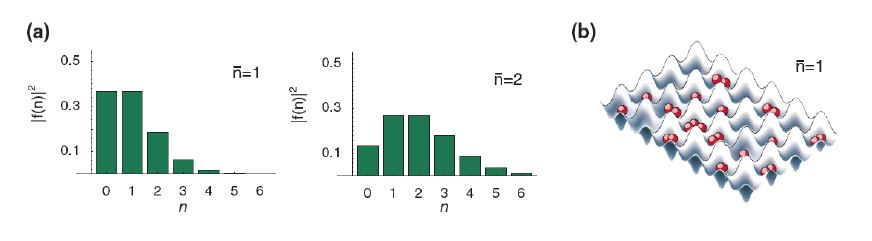
\includegraphics[width=0.8\columnwidth]{Figures/f(n)_SF.JPG} 
	\caption{(a)The statistics for the number of particles per lattice site $n$ for a filling fraction of $\bar{n}=1$ and $\bar{n}=2$ in the superfluid phase. (b) Illustration of the particles in the lattice. There will be large fluctuations of the number of particles found at each lattice site at a given time. \cite{greiner}}
	\label{fig:f(n)_SF} 
\end{figure}
For large systems the dispersion relation of the superfluid state (equation \ref{SFenergy}) is continues. In other words, the spectrum is \textit{gapless}, since excitations with any energy are possible.


\section{Mott-Insulator Phase}
In the case of very strong interactions the Hamiltonian reads
\begin{equation}
	\hat{H} = \hat{H}_U = \frac{U}{2} \sum_{i} \hat{n}_i \left( \hat{n}_i -1 \right) \; ,
	\label{hamilMott}
\end{equation}
which is quadratic in $\hat{n}_i$. This heavily penalizes having many particles at the same site. Thus, the ground state of the system will be an equal distribution of all the particles throughout the lattice. Any fluctuations from this average will increase the energy. This state is called the \textit{Mott Insulator}, and its statistics are illustrated in figure \ref{fig:f(n)_M}.\\
\begin{figure}[!h]
\centering
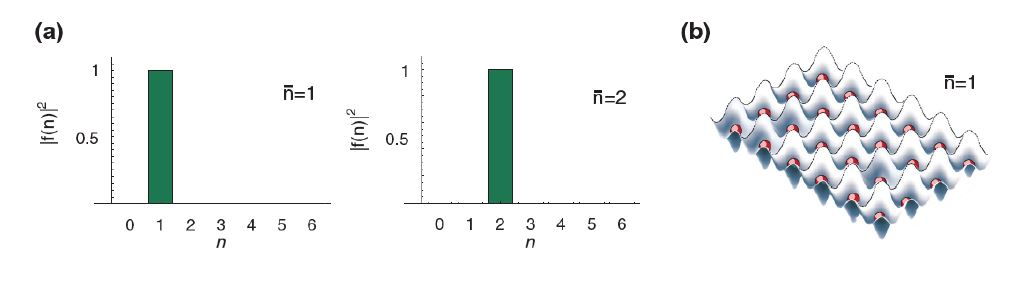
\includegraphics[width=0.8\columnwidth]{Figures/f(n)_M.JPG} 
\caption{(a)The statistics for the number of particles per lattice site $n$ in the Mott-insulator phase, for a filling fraction of $\bar{n}=1$ and $\bar{n}=2$. (b) Illustration of the particles in the lattice. The particles does not hop around in the lattice and are equally distributed. \cite{greiner}}
\label{fig:f(n)_M} 
\end{figure} 

Consider the case $\bar{n} = 1$, (average filling of one particle per site). This can be described by a state with a single particle located on each site \cite{manybodyBloch}
\begin{equation}
	\ket{\Psi_{Mott}} = \prod_j \hat{a}_{j}^{\dag} \ket{0} \; .
\end{equation}
From the Hamiltonian \ref{hamilMott} the energy of the state is zero. Any fluctuation from this average will increase the energy by $U$, which in the limit $J/U \rightarrow 0$ can be quite substantial. Hence, the ground state is stable against non-zero kinetic energies, prompting the name \textit{Insulator}. This complete isolation of the different wells of the lattice means that any phase coherence is lost. Furthermore, as opposed to the superfluid the spectrum of the Mott insulator is gapped, meaning that there exist a lowest excitation energy - in this case $U$.


\section{Phase Transition}
Consider once again the full Bose-Hubbard Hamiltonian \ref{BHhamil}. The superfluid and the Mott-Insulator account for the two limits of the ratio $J/U$, however, it order to understand the full phase diagram of the Bose-Hubbard model one has to derive the $U_{crit}$ for which the phase transition occurs. There are several ways of doing this - one of them is looking at a mean-field solution of the Bose-Hubbard model. For simplicity the scenario $T=0$ is treated here. Even without a change of temperature the phase transition still happens, hence the label \textit{quantum phase transition} referring to the fact that the phase transition can happen without change of external parameters.\\
Applying the mean field approximation to the annihilation operator yields
\begin{equation}
	\hat{a}_j = \psi + \delta \hat{a}_j \; ,
\end{equation}
where $\psi$ is the locally constant mean field, and $\delta \hat{a}_j$ is the fluctuation term. Inserting this into the Hamiltonian yields
\begin{equation}
	\hat{H}_{MF} = -J \sum_{\langle i,j \rangle} \left( \psi^* + \delta \hat{a}_{i}^{\dag} \right) \left( \psi + \delta \hat{a}_{j} \right) + \text{int.}
\end{equation}
Instead of considering the Hamiltonian as a whole, it can be considered as a sum of local on-site Hamiltonians
\begin{equation}
	\hat{H}_{MF} = \sum_{i} \hat{h}_i \; .
\end{equation}
For a homogeneous system $\hat{h}_i = \hat{h}_j \; \; \forall i,j$. One can write the kinetic part of the Hamiltonian locally if one assumes small fluctuations from the mean field
\begin{align}
  \hat{a}_{i}^{\dag} \hat{a}_{j} &= \left( \psi^* + \delta \hat{a}_{i}^{\dag} \right) \left( \psi + \delta \hat{a}_{j} \right) \nonumber \\
  &= \psi^* psi + \psi^* \delta \hat{a}_j + \psi \delta \hat{a}_{i}^{\dag} + \delta \hat{a}_{i}^{\dag} \delta \hat{a}_{j} \nonumber \\
  & \approx \psi^* psi + \psi^* \left( \hat{a}_j - \psi \right) + \psi \left( \hat{a}_{i}^{\dag} - \psi^* \right) \nonumber \\
&= \psi^* \hat{a}_j + \psi \hat{a}_{i}^{\dag} - \psi^* \psi
\end{align}
Since every term only contains a single index, one can let $j \rightarrow i$ leaving a local description
\begin{equation}
	\hat{h}_i = J z \psi^* \psi - J z \left( \psi^* \hat{a}_i + \psi \hat{a}_{i}^{\dag} \right) + \frac{U}{2} \hat{n}_i \left( \hat{n}_i -1 \right) + \mu_i \hat{n}_i \; ,
	\label{localhamil}
\end{equation}
where $z$ is the number of neighbours of site $i$ \cite{vanoosten}. The last term added is a chemical potential, which is needed due to the lack of a fixed particle number locally prompting the use of a Grand Canonical Ensemble description.\\
Landau theory is a general theory regarding phase transitions, which states that in the vicinity of a critical point, one may expand the free energy in a power series of some order parameter $m$. Thus, in order to find $U_{crit}$ \ref{localhamil} must be minimized. In this case this order parameter is the mean field, hence
\begin{equation}
	E_{MF} = \text{const. } + a |\psi|^2 + b |\psi|^4 + \ldots \label{eq:landau}
\end{equation} 
Plotting this yields an effective potential, seen in figure \ref{fig:landau}, which dictates certain properties of the system.
\begin{figure}[!h]
\centering
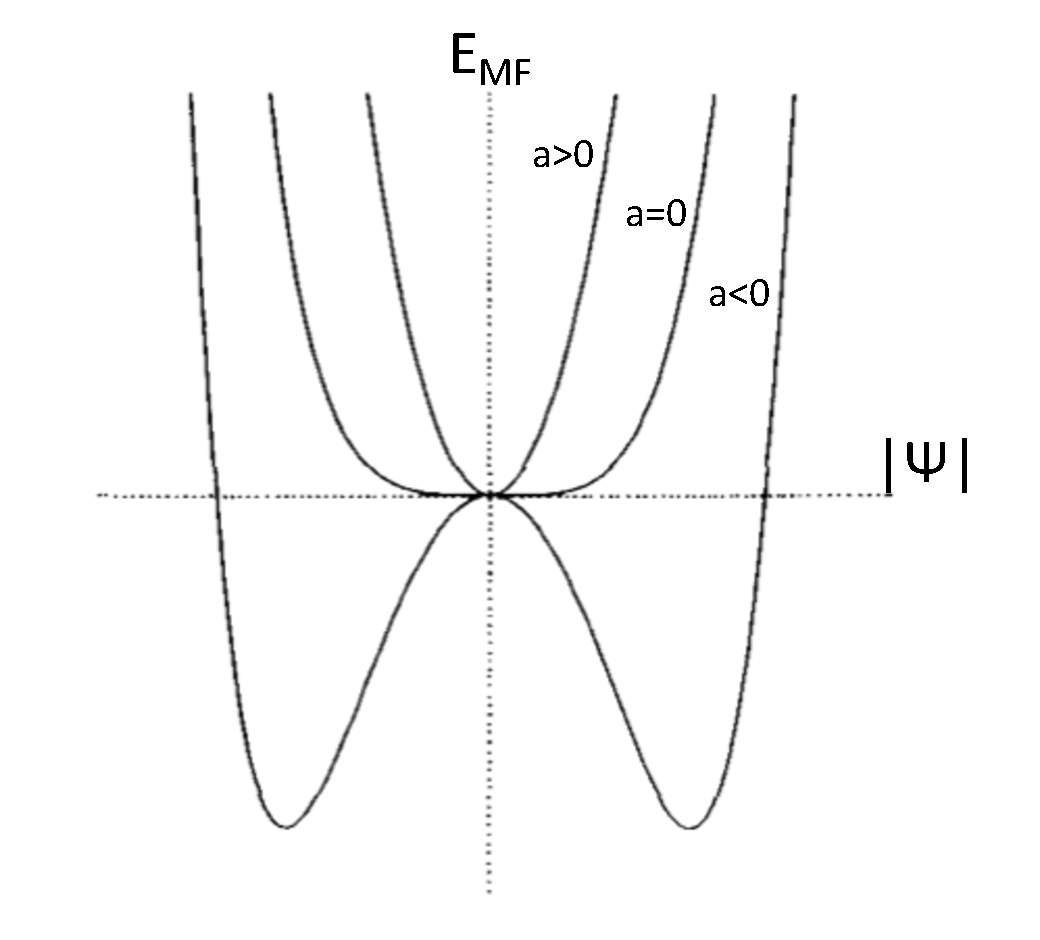
\includegraphics[width=0.7\columnwidth]{Figures/Landau_theory.pdf} 
\caption{	\textit{Effective potential as function of the order parameter $\psi$. For $a<0$ the properties of the potential change from having a single, central minimum to having two separated minima. This is an example of spontaneous symmetry breaking associated with a phase transition. \cite{plischke}}}
\label{fig:landau} 
\end{figure} 

The potential is symmetric in the complex plane allowing the system to have any phase. Furthermore, at some critical value of $a$, (here $a = 0$), the potential will shift from having a single central minimum to having minima at some $|\psi|$. This is a U(1) spontaneous symmetry breaking, which in Landau theory is associated with a phase transition \cite{plischke}. Thus, one need to compute the parameter $a$ of equation \ref{eq:landau}.\\
One method is using second order perturbation theory, where the $\hat{\psi} = 0$ case is solved exactly, followed by adding a small $\hat{\psi}$ as a perturbation
\begin{equation}
	\hat{h}_{i}^{(0)} = J z \left( \psi^* \psi \right) + \frac{U}{2} \hat{n}_i \left( \hat{n}_i -1 \right) - \mu \hat{n}_i \; .
\end{equation} 
Since the zero-order solution only contain number operators, the ground state of the solution can be expressed in the Fock basis:
\begin{align*}
	\ket{0} \quad &\text{for} \quad \mu < 0 \\
	\ket{1} \quad &\text{for} \quad 0 \leq \mu < U \\
	\ket{2} \quad &\text{for} \quad U \leq \mu < 2 U \\
	& \vdots
\end{align*} 
Adding on the first order perturbation to the energy
\begin{equation}
	E_{i}^{(1)} = \bra{n} \delta \hat{a}_i \ket{n} = 0 \; ,
\end{equation}
yields nothing, thus requiring the use of a second order perturbation
\begin{equation}
	E_{i}^{(2)} = \sum_{n \neq g} \frac{|\bra{n} \delta \hat{h}_i \ket{g}|^2}{E_{g}^{(0)} - E_{n}^{(0)}} \; .
\end{equation}
Here the perturbation Hamiltonian
\begin{equation}
	\hat{h}_i = - z J \left( \hat{a}_i \psi^* + \psi \hat{a}_{i}^{\dag} \right)
\end{equation}
contains only single creation/annihilation operators, whereby
\begin{equation}
	\bra{n} \delta \hat{h}_i \ket{g} = 0 \quad \text{for} \quad |n - g| \neq 1 \; .
\end{equation}
Hence, for each annihilation and creation operator only two matrix elements will give a contribution
\begin{align*}
	\bra{n}  \hat{a}_{i}^{\dag} \ket{n-1} &= \sqrt{n} \braket{n|n} \\
	\bra{n+1}  \hat{a}_{i}^{\dag} \ket{n} &= \sqrt{n+1} \braket{n|n} \\
	& \vdots
\end{align*}
With this the second order perturbation energy reduces to
\begin{align}
	E_{i}^{(2)} &= \left( J z \right)^2 |\psi|^2 \left( \frac{n}{E_{g}^{(0)}- E_{n-1}^{(0)}} +  \frac{n+1}{E_{n}^{(0)}- E_{n+1}^{(0)}} \right) \nonumber \\
	&= \left( J z \right)^2 |\psi|^2 \left( \frac{n}{U(n-1) - \mu} + \frac{n+1}{\mu - U n} \right) \; .
\end{align}
Since $a$ is the pre-factor of all terms proportional $|\psi|^2$, collecting those across from all the perturbations yields the approximation 
\begin{equation}
	a = J z + \left( J z \right)^2 |\psi|^2 \left( \frac{n}{U(n-1) - \mu} + \frac{n+1}{\mu - U n} \right) \; .
\end{equation} 
As stated earlier $U_{crit}$ can be found from $a = 0$:
\begin{equation}
	0 \overset{!}{=} 1 + \frac{n}{\bar{U} (n-1) - \bar{\mu}} + \frac{n+1}{\bar{\mu} - \bar{U} n} \; ,
\end{equation}
with $\bar{mu} = \frac{\mu}{J z}$ and $\bar{U} = \frac{U}{J z}$. Finally, the solution for the chemical potential is \cite{vanoosten}
\begin{equation}
	\bar{mu}_{\pm} = \frac{1}{2} \left( \bar{U}(2n -1) \pm \frac{1}{2} \sqrt{\bar{U}^2 - 2 \bar{U} (2 n +1)} \right) \; .
\end{equation}
Understanding this result can be done be examining figure \ref{fig:SFMOTT}, which displays a phase diagram of the Bose-Hubbard model.  
\begin{figure}[h]
	\centering
	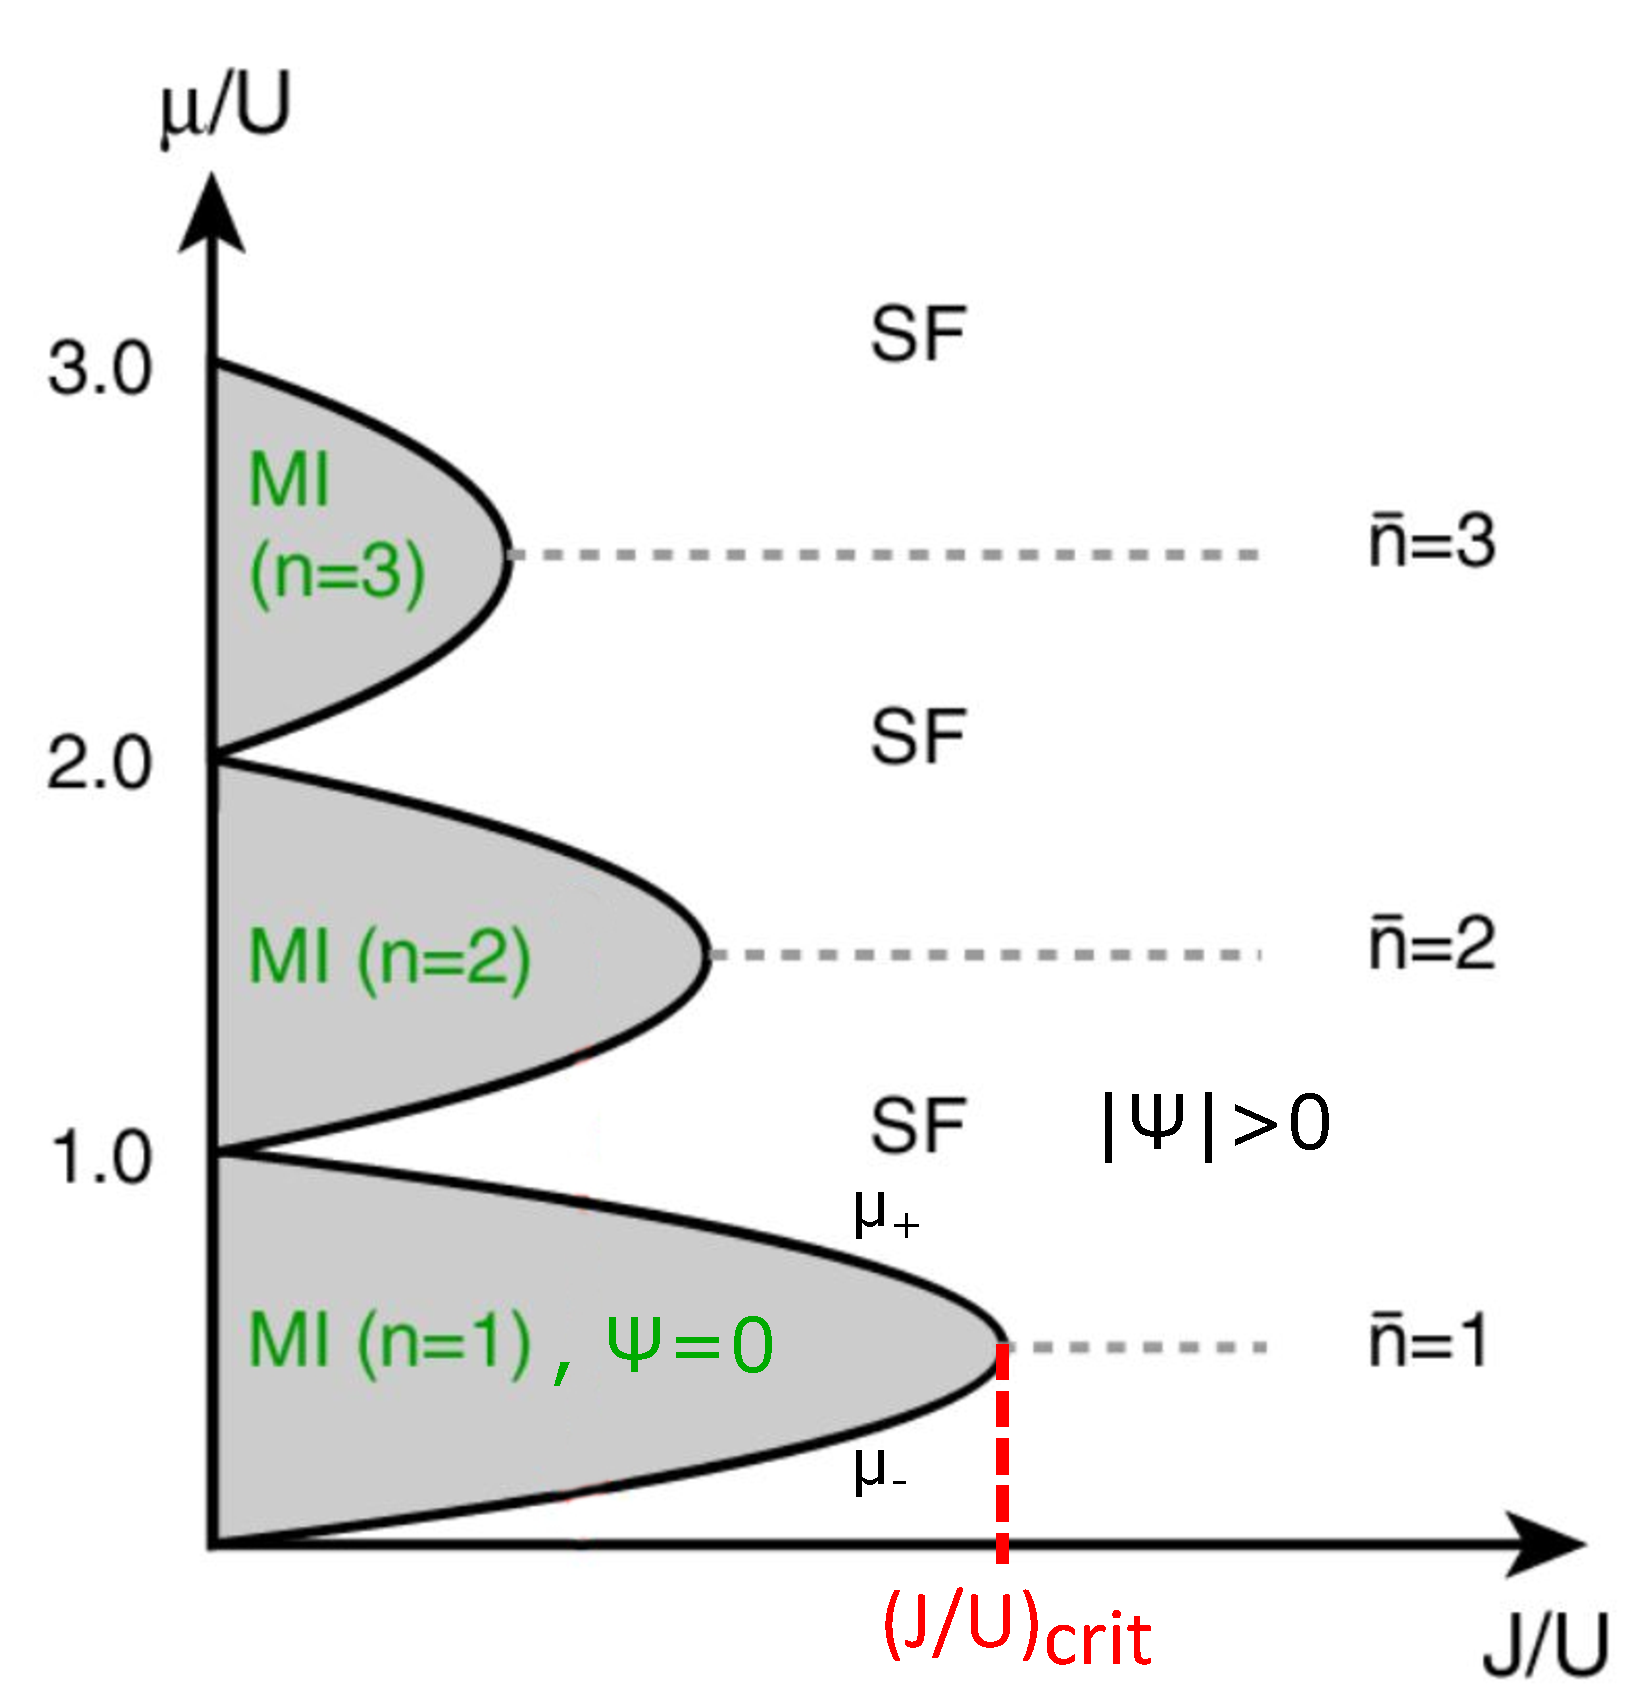
\includegraphics[width = 0.7\textwidth]{Figures/SFMottPhase.pdf}
	\label{fig:SFMOTT}
	\caption{\textit{Phase diagram of Bose-Hubbard model for T = 0. Grey areas mark the Mott Insulator phase for different number of particles per site, while white regions mark the superfluid phase. \cite{greiner}}}
\end{figure}
The $\mu_{\pm}$ curves encloses the region where the system is in the Mott Insulating phase. $(1/\bar{U})_{crit} = (J/U)_{crit}$ can be read off the graph from the point, where the two curves $\mu_{\pm}$ meet. As mentioned earlier, no fluctuations take place in the Mott Insulator, whereby the particle number per site is well defined, while it for the superfluid can take many values. As the chemical potential increases each site can accommodate more particles as long as the increase in chemical potential compensates the increased energy due to interactions between the particles.\\
The mean-field solution of the Bose-Hubbard model is only an approximation, which proves quite inaccurate for one dimension. This is seen when comparing the critical ratio for the mean-field approach, $\left( U/J \right)_{crit}^{MF,1D} = 11.66$, with numerical results computed using the DMRG method, $\left( U/J \right)_{crit}^{DMRG,1D} = 3.37$, \cite{Kuhner2000}. Nevertheless, it gives a good intuitive feeling of the physics taking place and how one can describe them without resorting to diagonalizing the Hamiltonian.\\